%% tez.tex
%% forked from github/gokcemay
%
% reformatted by Nuri Ozbey
% This work may be distributed and/or modified under the
% conditions of the LaTeX Project Public License, either version 1.3
% of this license or (at your option) any later version.
% The latest version of this license is in
%   http://www.latex-project.org/lppl.txt
%
%
% This work consists of the files esogu.cls and tez.tex




% Şablon otomatik olarak kapak ve onay sayfalarını sizin esogu.cls dosyasında girdiğiniz bilgilere göre oluşturmaktadır. Lütfen o dosyadaki "TEZLE İLGİLİ Bilgileri burada giriniz." bölümünü doldurunuz. 

% Eğer Tezinizi bu dosyada yazacaksanız "TEZİNİZİ BURADAN SONRA EKLEYİNİZ" bölümünden sonra ekeleyebilirsiniz. Özet ve Summary bölümleri /bolum klasörünün içindedir. 


\documentclass[]{esogu}			% Optionlar boş olacak, şablonu kullanmak için
\usepackage{lipsum}				% Örnek tezde anlamsız metin yazmak için bu paket gerekli. Tezinizde bu bölümü silebilirsiniz. 

\bibliography{kaynakca.bib}		% Kaynakça dosyası için Bunu Zotero, Mendeley, Endnote ya da CiteU gibi bir programla oluşturmanızı tavsiye ederim. Zotero hakkında bilgi http://makina.gmay.me/Bulutta/ adresindeki ekitapta mevcut.



%%%%%%%KISALTMALAR%%%%%%%%%%%%%%%%%%%
%% Kısaltmalar için lütfen glossaries paketine bakınız.
\newglossarystyle{mylong3col}{%
  \setglossarystyle{long3colheader}%
  \renewcommand\entryname{\underline{Kısaltmalar}}
  \renewcommand\descriptionname{\underline{Açıklama}}
  \renewcommand{\pagelistname}{\underline{}}
  \renewenvironment{theglossary}%
    {\begin{longtable}[l]{p{6cm}p{8cm}p{0.1cm}}}%
    {\end{longtable}}%
}

\makeglossaries

\newacronym{fer}{YYY}{Lorem ipsum dolor}
\newacronym{lbp}{YİÖ}{sit amet}
\newacronym{pca}{TBA}{ Ut purus elit }
\newacronym{svm}{DBW}{vestibulumHEADER}
\newacronym{sffs}{VBS}{vestibulum}
\newacronym{sbfs}{ASİ}{asi}
\newacronym{cva}{OCY}{OO char Axes}
\newacronym{rf}{ROE}{Rass Opram Eskrim}
\newacronym{logreg}{LTSS}{Lojistik Transport Service}
\newacronym{ann}{YSA}{Yes Supply Angle}

\newacronym{hog}{YGH}{You Gain Here}
\newacronym{ldp}{YYYD}{Yes You DO}
\newacronym{lmp}{Ymm}{Yes Massive Mass}
\newacronym{dke}{DKE}{Dj K Enred}
\newacronym{cnnetwork}{Cast}{Cast NBewst}
\newacronym{smote}{SWCU}{Some Watch Call Us}
%----------------------
\newacronym{hogEN}{HOG}{HOsGel}
\newacronym{lbpEN}{LBOPER}{Last Binary}
\newacronym{pcaEN}{PPP}{Prsssysis Prates }
\newacronym{svmEN}{SSSS}{SuVesdMultiplys}
\newacronym{sffsEN}{SDFFF}{Sefsadsfaweffffon}
\newacronym{sbfsEN}{SBAER}{Sesdfadfsbction}
\newacronym{cvaEN}{CART}{Casdaach}
\newacronym{rfEN}{RASTW}{Rsatt}
\newacronym{logregEN}{KLOW}{kloww}

\newacronym{ckplus}{CASST}{ CASTER - CANADIAN}

%\newacronym{pi}{$\pi$}{$\pi$ sayısı}








%----------------------------------------------------------------------------------------
\begin{document}

\frontmatter %roma rakamları ile yazdırmak için
\title{OGU deneme}
%-----Dış kapak Türkçe---------- Burayı değiştirmeyin
\begin{titlingpage*}
\begin{center}

\vspace*{8cm}								% Metnin yukarı mesafesi * olmazsa sayfa başında boşluk silinir
	\tbaslik\\								% Tez başlığı
	\vspace{1pc}							%12 punto boşluk ver
	\yazar	\\								% yazar ismi
	\vspace{1pc}							%12 punto boşluk ver
	\textbf{\unvan\space TEZİ}\\
    \vspace{1pc}							%12 punto boşluk ver
	\bolum \space Anabilim Dalı\\
    \vspace{1pc}							%12 punto boşluk ver
	\teslim\\
\end{center}

\end{titlingpage*}
%----------------------------------------------------------------------
%-----Dış kapak İngilizce-----Burayı değiştirmeyin-----
\begin{titlingpage*}
\begin{center}

\vspace*{8cm}
	\tbasliken\\								% Tez başlığı
	\vspace{1pc}
	\yazar	\\								% yazar ismi
	\vspace{1pc}
	\textbf{\unvanen}\\
  	\vspace{1pc}
	\bolumen \space Department\\
	\vspace{1pc}
	\teslimen\\
\end{center}

\end{titlingpage*}
%----------------------------------------------------------------------
%	iç Kapak Burayı değiştirmeyin
%----------------------------------------------------------------------------------------

\begin{titlingpage*}
\begin{center}
\vspace*{10mm}
\tbaslik\\								% Tez başlığı
\vspace{12pc}							% 12 punto 7 boşluk için
\yazar	\\								% yazar ismi
\vspace{8pc}							% 12 punto 7 boşluk için
Eskişehir Osmangazi Üniversitesi\\		
Fen Bilimleri Enstitüsü\\
Lisansüstü Yönetmeliği Uyarınca\\
\bolum \space Anabilim Dalı\\
\bilim \space Bilim Dalında\\
\unvan \space TEZİ\\
Olarak Hazırlanmıştır\\
\vspace{7pc}
Danışman:\space \danisman\\			
\vfill
%\proje\\ 								%Varsa proje kapsamında desteklenip desteklenmediği buraya yazılacak
\vspace{1pc}
\teslim\\
\vspace{2cm}
\end{center}

\end{titlingpage*}
\normalsize

%----------Onay--------------
\thispagestyle{empty}
\begin{center}
\large
\textbf{ONAY} 
\normalsize
\end{center}

\bolum \space Anabilim Dalı \unvan \space öğrencisi \yazar'ın \space \unvan\space tezi olarak hazırladığı "\textbf{\tbaslik}" başlıklı bu çalışma,\space jürimizce lisansüstü yönetmeliğin ilgili maddeleri uyarınca değerlendirilerek oybirliği ile kabul edilmiştir.
\vspace{15mm}

\noindent \textbf{Danışman}\space\space\space\space\space\space\space\space:\space \danisman 

\noindent \textbf{İkinci Danışman}\space:\space \ikidanisman
\newline

\noindent \textbf{Yüksek Lisans Tez Savunma Jürisi:}

\noindent \textbf{Üye :\space}\jbir

\noindent \textbf{Üye :\space}\jiki

\noindent \textbf{Üye :\space}\juc

\noindent \textbf{Üye :\space}\jdort

\noindent \textbf{Üye :\space}\jbes

\vspace{15mm}

\begin{framed}
Fen Bilimleri Enstitüsü Yönetim Kurulu'nun ........................ tarih ve  \space \space \space \space \space\\................... sayılı kararıyla onaylanmıştır. 
\newline
\newline
\begin{flushright}
\mudur \\
Enstitü Müdürü\space \space \space \space \space \space \space \space \space \space \space \space \space \space %Düzeltilecek ***Biliyorum çok kötü ama hspace çalışmadı
\end{flushright}

\end{framed}


%-------------------Şekiller ve Çizelgeler Dizini----------------
\renewcommand{\listfigurename}{ŞEKİLLER DİZİNİ}
\renewcommand{\listtablename}{ÇİZELGELER DİZİNİ}

\setlength\beforechapskip{-\baselineskip}


\normalsize
\begin{center}
\Large\textbf{ETİK BEYAN}
\end{center}
\normalsize
\vspace{3cm}

Eskişehir Osmangazi Üniversitesi Fen Bilimleri Enstitüsü tez yazım kılavuzuna göre, \danisman\space danışmanlığında hazırlamış olduğum “\textbf{\tbaslik}” başlıklı tezimin özgün bir çalışma olduğunu; tez çalışmamın tüm aşamalarında bilimsel etik ilke ve kurallara uygun davrandığımı; tezimde verdiğim bilgileri, verileri akademik ve bilimsel etik ilke ve kurallara uygun olarak elde ettiğimi; tez çalışmamda yararlandığım eserlerin tümüne atıf yaptığımı ve kaynak gösterdiğimi ve bilgi, belge ve sonuçları bilimsel etik ilke ve kurallara göre sunduğumu beyan ederim.   16/06/2022
\vspace{3cm}

\begin{flushright}
\yazar
\end{flushright}\thispagestyle{empty}
\clearpage

%Özette tez çalışmasının amacı, kapsamı, kullanılan yöntemler ve varılan sonuçlar açık ve öz olarak belirtilmeli, bunlar alt başlıklar altında sunulmamalıdır.  Özetin uzunluğu 250 kelimeyi geçmemelidir. 

%Summary sayfasının içeriği ve düzeni tümüyle Özet sayfasının aynı olmalı ve (vii) ile numaralanmalıdır.

%Özet ve Summary’nin altına anahtar kelimeler/keywords yazılmalıdır.  Konu literatürde hangi kelimelerle geçiyorsa anahtar kelime olarak bu kelimeler kullanılmalıdır.

\chapter{ÖZET}
\lipsum[1-2]

\noindent
\textbf{\textit{Anahtar Kelimeler:}}
\lipsum[7]
\chapter{SUMMARY}
\lipsum[7-9]


% Yüz ifadesi tanıma ve analiz etme son yıllarda popüler bir konu haline geldi. Önceden insan-makine etkileşimini, güvenlik, psikolojik analiz ve eğlence amaçlı kullanılırken, son zamanlarda web sitesi ve pazarlama uygulamaları ile sosyal medyada eğlence uygulamaları araştırmacıları bu konu üzerine çalışmaya yoğunlaştırdı. Literatürdeki çalışmalar artmasına rağmen bu konudaki tanıma hassasiyeti ve zorluğu halen devam etmekte. Bu konudaki çalışmaları ve tanımaları farklılaştıran en büyük etki insanın doğal yapısı gereği ortaya çıkan farklı ırklardaki farklı yüz tiplerinin oluşması olmuştur. Tek bir tipteki ifade tanıma başarısı çok iyi olmasına rağmen farklı tiplerde ortaya çıkan tanıma zorluğu halen bir yarış olarak devam etmektedir.

% Gerçekleştirilen bu tez çalışmasında literatürdeki yapılan çalışmalara ek yeni bir öznitelik çıkarımı ve veri seti üzerindeki dengeleme ile daha hassas ve daha başarılı bir yöntem önerilmiştir. Bu yöntemler kıyaslanırken video olarak geçmişe dayalı bir sınıflandırma yerine tek bir resim üzerinden sınıflandırma gerçekleştirilmeye çalışılmıştır. Çalışmanın ilk aşaması olarak ayırt edici özellik olarak öznitelik türetme ile başlamıştır. Bu aşamada üç farklı yöntem olarak, geometrik öznitelikler, \acrfull{hog} ve \acrfull{lbp} kullanılmıştır. Geometrik öznitelik türetme aşamasında, yeni yaklaşımlar önerilmiş ve bu öznitelikler türetilirken (Özbey ve Gülmezoğlu, 2021) çalışmasındaki yaklaşımlardan yararlanılmıştır. Deneysel çalışmalarda genişletilmiş \acrfull{ckplus} veri kümesi kullanılmış ve yüz ifadeleri 10 katlı çapraz doğrulama yöntemi kullanılarak 4 farklı sınıflandırıcı; \acrfull{svm}, \acrfull{rf},\acrfull{logreg} ve \acrfull{cva} ile sınıflandırılmıştır. Sınıflandırma başarısını arttırmak için \acrfull{sffs} , \acrfull{sbfs} ve \acrfull{pca} ile öznitelik azaltma işlemi yapılmıştır. 

\noindent
\textbf{\textit{Keywords:}}
One, two, three, four, five
\chapter{TEŞEKKÜR}
\lipsum[15]

% \addto\captionturkish{% Büyük harfle olması için
%   \renewcommand{\contentsname}%
%     {İÇİNDEKİLER}%
% }
\renewcommand{\contentsname}%
    {İÇİNDEKİLER}%

\newcommand\MyShipoutHook{\chapter*{\contentsname \MakeLowercase{{ (devam)}}}}
\AtBeginShipout{\MyShipoutHook}
\tableofcontents
\renewcommand\MyShipoutHook{}
\newpage


\newcommand\MyShipoutHooknn{\chapter*{ŞEKİLLER DİZİNİ \MakeLowercase{{ (devam)}}}}

\AtBeginShipout{\MyShipoutHooknn}
\listoffigures
\renewcommand\MyShipoutHooknn{}
\newpage
\listoftables

\clearpage


\printglossary[style=mylong3col, type=\acronymtype, title=Simgeler ve Kısaltmalar Dizini, toctitle=SİMGELER VE KISALTMALAR DİZİNİ,nonumberlist]
\clearpage
% \renewcommand{\listtheoremname}{TEOREMLER DİZİNİ}
% \listoftheorems[ignoreall,onlynamed={theorem}]
% \clearpage
% \renewcommand{\listtheoremname}{İSPATLAR DİZİNİ}
% \listoftheorems[ignoreall, show={ispat}]
% \clearpage

\mainmatter %arap harfleri ile yazdırmak için
% AltBölüm numaralaması
\setcounter{secnumdepth}{5} % 5 derine kadar numara ver.
%---------TEZİNİZİ BURADAN SONRA EKLEYİNİZ-----------------


\chapter{GİRİŞ}



Basit iki terimle \acrfull{lbp} ve \acrfull{svm} kısaltmaları anlatabiliriz. İster kısaltmasını \acrshort{svm}, isterseniz de uzun açılımını \acrlong{svm} yazdırabilirsiniz. Bunu yapabilmek için dosyanın başında terimleri tanımlamanız gereklidir. İsterseniz matematik terimlerini de, örneğin \acrshort{pca} böyle tanımlayabilirsiniz. Uzun uzun \acrfull{pca} yazmanız gerekmez. 
\acrfull{svm}
\acrshort{lbp}
\lipsum[16-20]
68 farklı noktanın konumları Şekil-\ref{fig:68point}'de gösterilmiştir.
\lipsum[3]
Öznitelik seçimi için boyut indirgeme aracı olan \acrfull{pca} , \acrfull{sffs} ve \acrfull{sbfs} uygulanmıştır.  
\begin{figure}[ht]
\centering
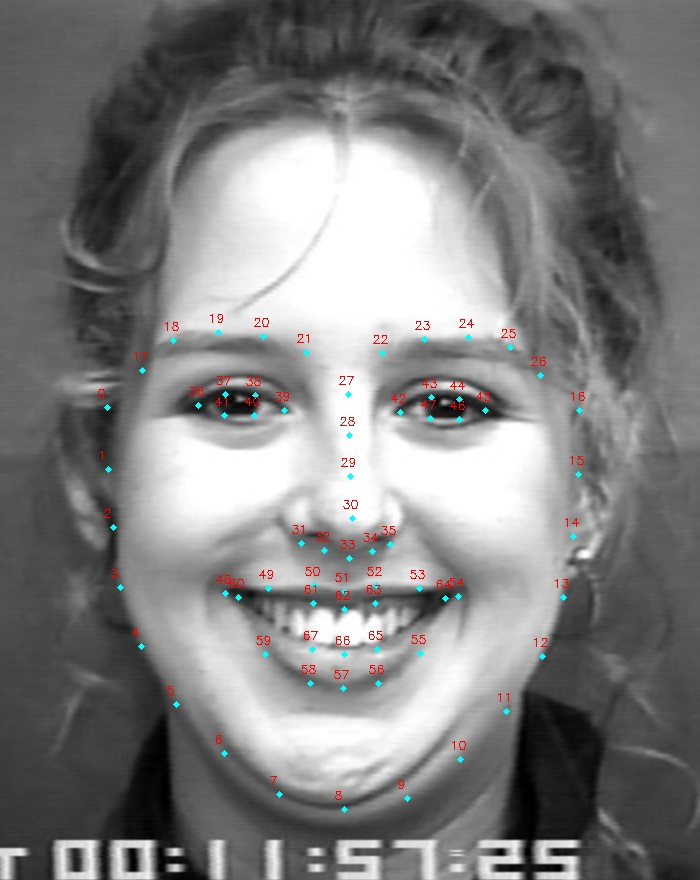
\includegraphics[trim={2cm 1.5cm 2cm 8cm},clip,width=0.75\textwidth]{gorseller/68point.jpg}
\caption{Nirengi Noktaları}\label{fig:68point}
\end{figure}
%[trim={5cm 0 0 0},clip] <left> <lover> <right> <upper>

\lipsum[5-8]

% Teorem yazmak isterseniz:
% \begin{theorem}[Öklid]
%  İki noktadan bir ve yalnız bir doğru geçer.
% \end{theorem}

% İspat yazmak isterseniz:
% \begin{ispat}[Tezin en önemli ispatı]
% x=10
% \end{ispat}
% \lipsum[1-2]
% \begin{figure}[h]
% \centering
% 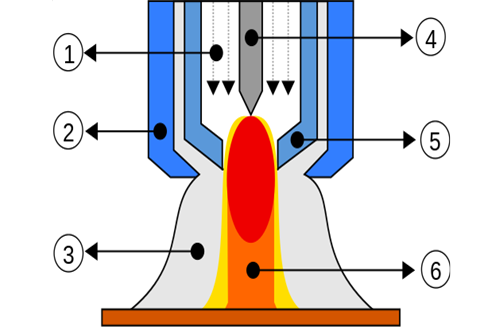
\includegraphics[width=\textwidth]{gorseller/ptaTorc}
% \caption{PTA Torç}\label{fig:PtaTorc1}
% \end{figure}
% \lipsum[1-2]
% \begin{table}
% \centering
% \caption{Deneme Tablosu.}\label{tab:den1}
% \begin{tabular}{|l|l|l|}
% \hline
% sıra   & sayı   & toplam \\ \hline
% 1      & 2      & 3      \\ \hline
% Kelime & deneme & son    \\ \hline
% \end{tabular}
% \end{table}


% %\section{Giriş Birinci Derece Başlık}
% \lipsum[1-2]
% \begin{figure}[h]
% \centering
% 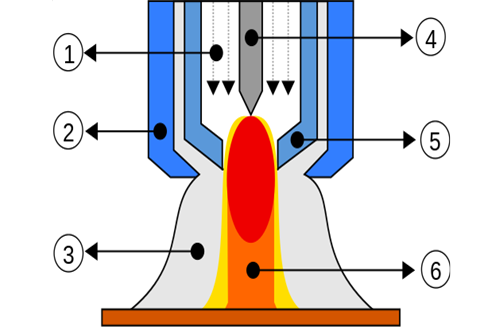
\includegraphics[width=\textwidth]{gorseller/ptaTorc}
% \caption{PTA Torç}\label{fig:PtaTorc1}
% \end{figure}
% \lipsum[1-2]
% \begin{table}
% \centering
% \caption{Deneme Tablosu.}\label{tab:den1}
% \begin{tabular}{|l|l|l|}
% \hline
% sıra   & sayı   & toplam \\ \hline
% 1      & 2      & 3      \\ \hline
% Kelime & deneme & son    \\ \hline
% \end{tabular}
% \end{table}
% Teorem yazmak isterseniz:
% \begin{theorem}[Öklid]
%  İki noktadan bir ve yalnız bir doğru geçer.
% \end{theorem}

% İspat yazmak isterseniz:
% \begin{ispat}[Tezin en önemli ispatı]
% x=10
% \end{ispat}

% %\subsection{Giriş ikinci derece başlık}
% \lipsum[1-2]
% \begin{figure}[h]
% \centering
% 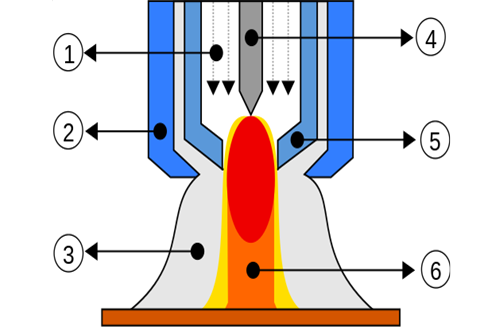
\includegraphics[width=\textwidth]{gorseller/ptaTorc}
% \caption{PTA Torç}\label{fig:PtaTorc1}
% \end{figure}
% \lipsum[1-2]
% \begin{table}
% \centering
% \caption{Deneme Tablosu.}\label{tab:den1}
% \begin{tabular}{|l|l|l|}
% \hline
% sıra   & sayı   & toplam \\ \hline
% 1      & 2      & 3      \\ \hline
% Kelime & deneme & son    \\ \hline
% \end{tabular}
% \end{table}

% Teorem yazmak isterseniz:
% \begin{theorem}[Öklid]
%  İki noktadan bir ve yalnız bir doğru geçer.
% \end{theorem}

% İspat yazmak isterseniz:
% \begin{ispat}[Tezin en önemli ispatı]
% x=10
% \end{ispat}

% %\subsubsection{Giriş dördüncü derece başlık}
% \lipsum[1-2]
% \begin{figure}[h]
% \centering
% 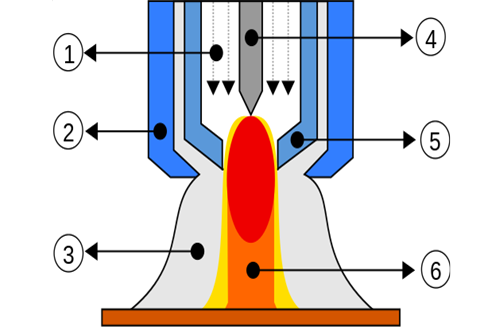
\includegraphics[width=\textwidth]{gorseller/ptaTorc}
% \caption{PTA Torç}\label{fig:PtaTorc1}
% \end{figure}
% \lipsum[1-2]
% \begin{table}
% \centering
% \caption{Deneme Tablosu.}\label{tab:den1}
% \begin{tabular}{|l|l|l|}
% \hline
% sıra   & sayı   & toplam \\ \hline
% 1      & 2      & 3      \\ \hline
% Kelime & deneme & son    \\ \hline
% \end{tabular}
% \end{table}

% Teorem yazmak isterseniz:
% \begin{theorem}[Öklid]
%  İki noktadan bir ve yalnız bir doğru geçer.
% \end{theorem}

% İspat yazmak isterseniz:
% \begin{ispat}[Tezin en önemli ispatı]
% x=10
% \end{ispat}				% Metni dosyadan çağırmak için örnek
\chapter{LİTERATÜR ARAŞTIRMASI}

\lipsum[6]
\parencite{shanvd2005}. 
\lipsum[7] 
\parencite{Zhaopaper}. 
\lipsum[5]
\parencite{he_chen}. 
\lipsum[8]
\acrfull{ldp}, \acrfull{lmp}, \acrfull{lbp} ve \acrfull{hog} çokça kullanılmıştır.

\parencite{barlett} 
\lipsum[10]
\acrfull{svm}  \acrfull{svm} dayalı özellik entegrasyonu ile birleştirerek bir yöntem sundular . 
%(Mohammad ve Ali, 2011),
\parencite{mohammad} çalışmalarında, \acrshort{lmp} yöntemini kullanmışlardır
% (Shan vd., 2009)
\parencite{SHAN2009}   \acrshort{lbp}  \acrshort{svm} 

\lipsum[11]


% (Zhao ve Zhang, 2011)
\parencite{zhaoandother}, Pellentesque habitant morbi tristique senectus et netus et malesuada fames ac turpis egestas.
%(Akyol ve Şahin, 2016),
\parencite{akyol} Donec odio elit, dictum in, hendrerit sit amet, egestas sed, leo. Praesent feugiat
sapien aliquet odio. Integer vitae justo
% (Gacav vd., 2018)
\parencite{gacav2018} Integer vitae justo. Aliquam vestibulum fringilla lorem. Sed neque
lectus, consectetuer at.
% (He ve Chen, 2020) 
\parencite{he_chen} Proin eu metus. Sed porttitor. In hac habitasse platea dictumst. Suspendisse eu
lectus.
% (Özbey ve Topal, 2018)
\parencite{ozbey2018}, Suspendisse vel felis. Ut lorem lorem, interdum eu, tincidunt sit amet, laoreet vitae, arcu. Aenean faucibus pede eu ante
% (Akcakoca ve Gökmen, 2015)
\parencite{akcakoca}, Quisque vehicula, urna sed ultricies auctor, pede lorem egestas dui, et convallis
elit erat sed nulla.
%(Bayrakdar vd., 2016)
\parencite{bayrakdar2017} Fusce mauris. Vestibulum luctus nibh at lectus. Sed bibendum, nulla a faucibus
semper, leo velit ultricies tellus 

Vivamus viverra fermentum felis. Donec nonummy pellentesque ante. Phasellus
adipiscing semper eli
%(Soyel ve Demirel, 2008)
\parencite{soyeldemirel} Nulla ac nisl. Nullam urna nulla, ullamcorper in, interdum sit amet, gravida ut, risus. Aenean ac enim \%88.5 Nullam urna.
\parencite{Ghimire_2013} vivamus viverra fermentum felis. Donec nonummy pellentesque ante. Phasellus
adipiscing semper elir.  

%(Gacav vd., 2016)
\parencite{gacav2016} Nulla ac nisl. Nullam urna nulla, ullamcorper in, interdum sit amet, gravida ut, risus. Aenean ac enim \%88.5 Nullam urna.
2017 yılında \parencite{Gacav2017} Nulla ac nisl. Nullam urna nulla, ullamcorper in, interdum sit amet, gravida ut, risus. Aenean ac enim \%88.5 Nullam urna.
\parencite{aksoy2016} Quisque vehicula, urna sed ultricies auctor, pede lorem egestas dui, et convallis
 \acrfull{dke} elit erat sed nulla. \acrshort{dke} Sed feugiat. Cum sociis natoque penatibus et magnis dis parturient montes, nascetur
ridiculus mus.
 
\acrfull{cnnetwork}, yüz ifadesi tanıma için kullanılan bir başka popüler yöntemdir ve geleneksel öznitelik çıkartma yöntemlerine kıyasla bu alandaki çalışmalarda kulanımı giderek artmaktadır. 
%(Tümen vd.,2017) 
\parencite{tumen2017}  Ut lectus eros, malesuada sit amet, fermentum eu, sodales cursus, magna \acrshort{cnnetwork}  \%57.1 Aenean faucibus pede eu ante.

% (Li vd.,2017) 
\parencite{li2017}  Integer arcu est, nonummy in, fermentum faucibus.
% (Abanoz ve Çataltepe, 2018)
\parencite{abanoz2018} Mauris felis odio.

% (Akay ve Arıca, 2018) 
\parencite{akayarıca2018} Suspendisse vel felis. Ut lorem lorem, interdum eu, tincidunt sit amet, laoreet vitae,arcu.
% (Liu vd.,2020) (Feng ve Shao, 2020)
\parencite{liu2020}, Donec pellentesque, erat ac sagittis semper, nunc dui lobortis purus, quis
congue purus metus ultricies tellus \acrshort{svm}, \parencite{fengshao2020} , Proin et quam. Class aptent taciti sociosqu. 
% (Videla ve Kumar, 2020)
\parencite{videlakumar2020} nubia nostra, per inceptos hymenaeos.
% (Mohan vd. 2020)
\parencite{mohan2021} Class aptent taciti sociosqu ad litora torquent per conubia nostra, per inceptos hymenaeos.



% Basit iki terimle \acrfull{OBEB} ve \acrfull{OKEK} kısaltmaları anlatabiliriz. İster kısaltmasını \acrshort{OBEB}, isterseniz de uzun açılımını \acrlong{OKEK} yazdırabilirsiniz. Bunu yapabilmek için dosyanın başında terimleri tanımlamanız gereklidir. İsterseniz matematik terimlerini de, örneğin \acrshort{pi} böyle tanımlayabilirsiniz. Uzun uzun \acrfull{pi} yazmanız gerekmez. 

% Teorem yazmak isterseniz:
% \begin{theorem}[Öklid]
%  İki noktadan bir ve yalnız bir doğru geçer.
% \end{theorem}

% İspat yazmak isterseniz:
% \begin{ispat}[Tezin en önemli ispatı]
% x=10
% \end{ispat}
% \lipsum[1-2]
% \begin{figure}[h]
% \centering
% 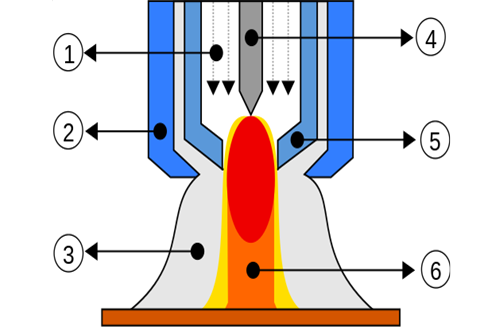
\includegraphics[width=\textwidth]{gorseller/ptaTorc}
% \caption{PTA Torç}\label{fig:PtaTorc1}
% \end{figure}
% \lipsum[1-2]
% \begin{table}
% \centering
% \caption{Deneme Tablosu.}\label{tab:den1}
% \begin{tabular}{|l|l|l|}
% \hline
% sıra   & sayı   & toplam \\ \hline
% 1      & 2      & 3      \\ \hline
% Kelime & deneme & son    \\ \hline
% \end{tabular}
% \end{table}


% % \section{Literatür Araştırması Birinci Derece Başlık}
% % \lipsum[1-2]
% \begin{figure}[h]
% \centering
% 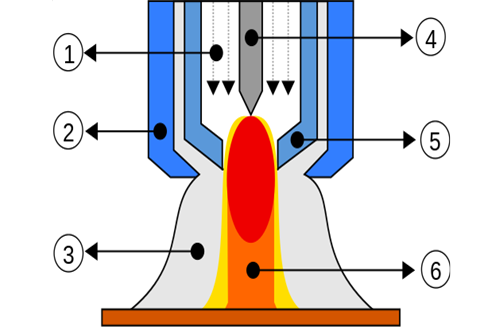
\includegraphics[width=\textwidth]{gorseller/ptaTorc}
% \caption{PTA Torç}\label{fig:PtaTorc1}
% \end{figure}
% \lipsum[1-2]
% \begin{table}
% \centering
% \caption{Deneme Tablosu.}\label{tab:den1}
% \begin{tabular}{|l|l|l|}
% \hline
% sıra   & sayı   & toplam \\ \hline
% 1      & 2      & 3      \\ \hline
% Kelime & deneme & son    \\ \hline
% \end{tabular}
% \end{table}
% Teorem yazmak isterseniz:
% \begin{theorem}[Öklid]
%  İki noktadan bir ve yalnız bir doğru geçer.
% \end{theorem}

% İspat yazmak isterseniz:
% \begin{ispat}[Tezin en önemli ispatı]
% x=10
% \end{ispat}

% % \subsection{Literatür Araştırması ikinci derece başlık}
% % \lipsum[1-2]
% \begin{figure}[h]
% \centering
% 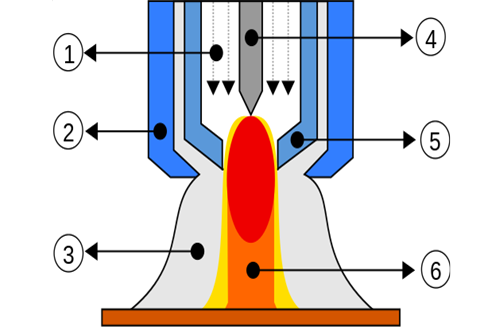
\includegraphics[width=\textwidth]{gorseller/ptaTorc}
% \caption{PTA Torç}\label{fig:PtaTorc1}
% \end{figure}
% \lipsum[1-2]
% \begin{table}
% \centering
% \caption{Deneme Tablosu.}\label{tab:den1}
% \begin{tabular}{|l|l|l|}
% \hline
% sıra   & sayı   & toplam \\ \hline
% 1      & 2      & 3      \\ \hline
% Kelime & deneme & son    \\ \hline
% \end{tabular}
% \end{table}

% Teorem yazmak isterseniz:
% \begin{theorem}[Öklid]
%  İki noktadan bir ve yalnız bir doğru geçer.
% \end{theorem}

% İspat yazmak isterseniz:
% \begin{ispat}[Tezin en önemli ispatı]
% x=10
% \end{ispat}

% % \subsubsection{Literatür araştırması dördüncü derece başlık}
% \lipsum[1-2]
% \begin{figure}[h]
% \centering
% 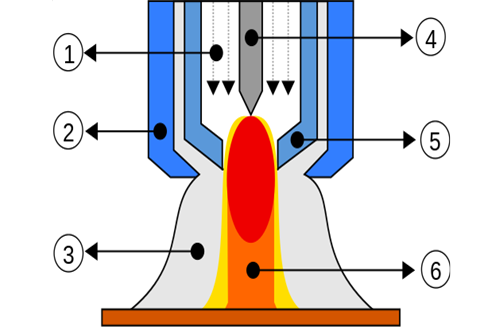
\includegraphics[width=\textwidth]{gorseller/ptaTorc}
% \caption{PTA Torç}\label{fig:PtaTorc1}
% \end{figure}
% \lipsum[1-2]
% \begin{table}
% \centering
% \caption{Deneme Tablosu.}\label{tab:den1}
% \begin{tabular}{|l|l|l|}
% \hline
% sıra   & sayı   & toplam \\ \hline
% 1      & 2      & 3      \\ \hline
% Kelime & deneme & son    \\ \hline
% \end{tabular}
% \end{table}

% Teorem yazmak isterseniz:
% \begin{theorem}[Öklid]
%  İki noktadan bir ve yalnız bir doğru geçer.
% \end{theorem}

% İspat yazmak isterseniz:
% \begin{ispat}[Tezin en önemli ispatı]
% x=10
% \end{ispat}
\chapter{MATERYAL VE YÖNTEM}



% Basit iki terimle \acrfull{OBEB} ve \acrfull{OKEK} kısaltmaları anlatabiliriz. İster kısaltmasını \acrshort{OBEB}, isterseniz de uzun açılımını \acrlong{OKEK} yazdırabilirsiniz. Bunu yapabilmek için dosyanın başında terimleri tanımlamanız gereklidir. İsterseniz matematik terimlerini de, örneğin \acrshort{pi} böyle tanımlayabilirsiniz. Uzun uzun \acrfull{pi} yazmanız gerekmez. 

% Teorem yazmak isterseniz:
% \begin{theorem}[Öklid]
%  İki noktadan bir ve yalnız bir doğru geçer.
% \end{theorem}

% İspat yazmak isterseniz:
% \begin{ispat}[Tezin en önemli ispatı]
% x=10
% \end{ispat}
% \lipsum[1-2]
% \begin{figure}[h]
% \centering
% 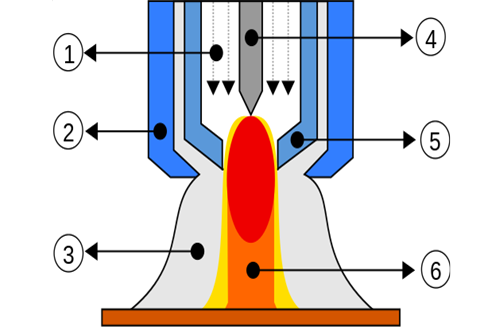
\includegraphics[width=\textwidth]{gorseller/ptaTorc}
% \caption{PTA Torç}\label{fig:PtaTorc1}
% \end{figure}
% \lipsum[1-2]
% \begin{table}
% \centering
% \caption{Deneme Tablosu.}\label{tab:den1}
% \begin{tabular}{|l|l|l|}
% \hline
% sıra   & sayı   & toplam \\ \hline
% 1      & 2      & 3      \\ \hline
% Kelime & deneme & son    \\ \hline
% \end{tabular}
% \end{table}


\section{Veri Kümesi}


\subsection{Haple Pasite Caseto Harra veri kümesi}
% \lipsum[1-2]
% \begin{table}[!bp]
% \centering
% \caption{CK+ veri setindeki her sınıf için örnek sayısı}
% \label{tab:datasetclasses}
% \begin{tabular}{|l|l|l|}
% \hline
% sıra   & sayı   & toplam \\ \hline
% 1      & 2      & 3      \\ \hline
% Kelime & deneme & son    \\ \hline
% \end{tabular}
% \end{table}


\lipsum[5-6]

\begin{figure}[ht]
\centering
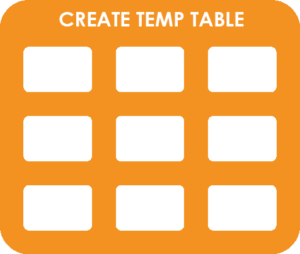
\includegraphics[width=0.99\textwidth]{gorseller/Temporary-Table.PNG}
\caption{wsdwwww}\label{fig:ckexample}
\end{figure}

\lipsum[6]. Çizelge\ref{tab:datasetclasses}'de.


\begin{table}[ht]
	\centering
	\tabulinesep=1mm
	\caption{Haple Pasite Caseto Harra veri kümesindeki her sınıf için örnek sayısı}
	\vspace{15mm}
	\newcommand{\tablecolumnsize}{0.075\columnwidth}
	
	{\normalsize 
		\begin{tabu} {
				>{\centering}m{\tablecolumnsize}
				>{\centering}m{\tablecolumnsize}
				>{\centering}m{\tablecolumnsize}
				>{\centering}m{\tablecolumnsize}
				>{\centering}m{\tablecolumnsize}
				>{\centering}m{\tablecolumnsize}
				>{\centering}m{\tablecolumnsize}
				>{\centering}m{\tablecolumnsize}
			}
			\begin{rotate}{45} sub1 \end{rotate} &
			\begin{rotate}{45} sub2 \end{rotate} &
			\begin{rotate}{45} sub3 \end{rotate} &
			\begin{rotate}{45} sub4 \end{rotate} &
			\begin{rotate}{45} sub5 \end{rotate} &
			\begin{rotate}{45} sub6 \end{rotate} &
			\begin{rotate}{45} sub7 \end{rotate} &
			\begin{rotate}{45} \textbf{Toplam} \end{rotate} \\
			\tabucline[1.5pt]{-}
			901 & 82 & 1582 & 121 & 1328 & 111 & 321 & \textbf{4122}
		\end{tabu}
	}
	
	\label{tab:datasetclasses}
\end{table}

\subsection{OPLE Cople Gubele Heo port}

\lipsum[19]
yöntem \parencite{Chawla_2002} 
\lipsum[16]
Çizelge-\ref{tab:smotetablo}'de verilmiştir. 

\begin{table}
\centering
\caption{Veri kümesindeki vektor sayıları}\label{tab:smotetablo}
\begin{tabular}{|l|l|l|}
\hline
\textbf{Sınıf}   & \textbf{Veri1}   & \textbf{Veri2} \\ \hline
sub1      & 231    & 355      \\ \hline
sub2 & 822 & 355    \\ \hline
sub3 & 165 & 355    \\ \hline
sub4 & 452 & 355    \\ \hline
sub5 & 312 & 355    \\ \hline
sub6 & 122 & 355    \\ \hline
sub7 & 322 & 355    \\ \hline
Toplam & 3135 & 3135    \\ \hline
\end{tabular}
\end{table}

% \begin{table}[ht]
% 	\centering
% 	\tabulinesep=1mm
% 	\caption{CK+ Veri Kümesi için SAAÖT Algoritması Uygulandığındaki Örnek Dağılımı}
% 	\vspace{10mm}
% 	\newcommand{\tablecolumnsize}{0.075\columnwidth}
	
% 	{\normalsize 
% 		\begin{tabu} {
% 				>{\centering}m{\tablecolumnsize}
% 				>{\centering}m{\tablecolumnsize}
% 				>{\centering}m{\tablecolumnsize}
% 				>{\centering}m{\tablecolumnsize}
% 				>{\centering}m{\tablecolumnsize}
% 				>{\centering}m{\tablecolumnsize}
% 				>{\centering}m{\tablecolumnsize}
% 				>{\centering}m{\tablecolumnsize}
% 			}
% 			\begin{rotate}{45} Öfke \end{rotate} &
% 			\begin{rotate}{45} Küçümseme \end{rotate} &
% 			\begin{rotate}{45} İğrenme \end{rotate} &
% 			\begin{rotate}{45} Korku \end{rotate} &
% 			\begin{rotate}{45} Mutluluk \end{rotate} &
% 			\begin{rotate}{45} Üzüntü \end{rotate} &
% 			\begin{rotate}{45} Şaşırma \end{rotate} &
% 			\begin{rotate}{45} \textbf{Toplam} \end{rotate} \\
% 			\tabucline[1.5pt]{-}
% 			166 & 166 & 166 & 166 & 166 & 166 & 166 & \textbf{1162}
% 		\end{tabu}
% 	}
	
% 	\label{tab:smoteclasses}
% \end{table}

% \subsection{Bulgular ve Tartışma ikinci derece başlık}
% \lipsum[1-2]
% \begin{figure}[h]
% \centering
% 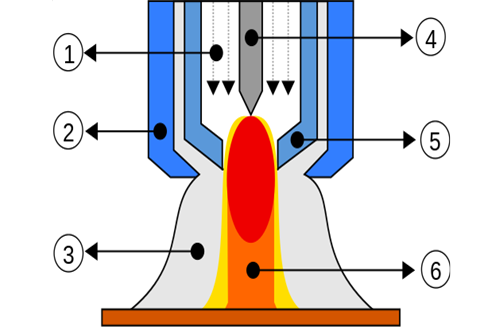
\includegraphics[width=\textwidth]{gorseller/ptaTorc}
% \caption{PTA Torç}\label{fig:PtaTorc1}
% \end{figure}
% \lipsum[1-2]
% \begin{table}
% \centering
% \caption{Deneme Tablosu.}\label{tab:den1}
% \begin{tabular}{|l|l|l|}
% \hline
% sıra   & sayı   & toplam \\ \hline
% 1      & 2      & 3      \\ \hline
% Kelime & deneme & son    \\ \hline
% \end{tabular}
% \end{table}

% Teorem yazmak isterseniz:
% \begin{theorem}[Öklid]
%  İki noktadan bir ve yalnız bir doğru geçer.
% \end{theorem}

% İspat yazmak isterseniz:
% \begin{ispat}[Tezin en önemli ispatı]
% x=10
% \end{ispat}

% \subsubsection{Bulgular ve tartışma dördüncü derece başlık}
% \lipsum[1-2]
% \begin{figure}[h]
% \centering
% 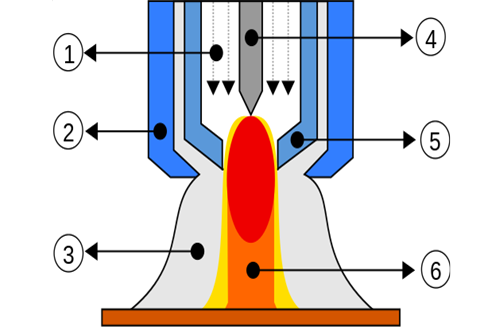
\includegraphics[width=\textwidth]{gorseller/ptaTorc}
% \caption{PTA Torç}\label{fig:PtaTorc1}
% \end{figure}
% \lipsum[1-2]
% \begin{table}
% \centering
% \caption{Deneme Tablosu.}\label{tab:den1}
% \begin{tabular}{|l|l|l|}
% \hline
% sıra   & sayı   & toplam \\ \hline
% 1      & 2      & 3      \\ \hline
% Kelime & deneme & son    \\ \hline
% \end{tabular}
% \end{table}

% Teorem yazmak isterseniz:
% \begin{theorem}[Öklid]
%  İki noktadan bir ve yalnız bir doğru geçer.
% \end{theorem}

% İspat yazmak isterseniz:
% \begin{ispat}[Tezin en önemli ispatı]
% x=10
% \end{ispat}
% Eğer metin içinde \(\lim_{x \to \infty} \exp(-x) = 0\) ya da ortalayabilir
% \begin{displaymath}
% \cos (2\theta) = \cos^2 \theta - \sin^2 \theta
% \end{displaymath}
% isterseniz de numaralı denklem yazabilirsiniz.

% \begin{equation}
% \frac{\mathrm d}{\mathrm d x} \left( k g(x) \right)
% \end{equation}
% \subsubsection{Kimya}
% \ce{B4C} yazabilirsiniz. Ya da

% \ce{CO2 + C -> 2CO}

% Daha fazlası için mhchem paketine bakınız.
 
% Eğer metin içinde şekile referans vermek isterseniz Şekil\ref{fig:68point} yazarsınız. 

% Kaynakça böyle verilebilir \parencite{celik_microstructure_2013} ya da iki yazarlı ise böyle verilebilir \parencite{gatto_plasma_2004} veya ikiden fazla ise böyle verilebilir.
% \parencite{celik_effects_2011}

% Kaynakça listesi için daha çok referans verilmek istenirse \parencite{yazdi_microstructure_2015, keehan_influence_2006, guo_microstructure_2014}, \parencite{kim_variation_2013}, bir başkası \parencite{xibao_metallurgical_2005},  ya da başkası \parencite{jin_effect_1997} kullanılabilir.

\section{Yöntem}


\lipsum[14-16]
\acrshort{lbp} \acrshort{hog} .


\lipsum[18-20] Şekil-\ref{fig:flowchart} da verilmiştir.


\begin{figure}[hp]
\centering

\begin{tikzpicture}[node distance=2cm]

\node (start) [startstop] {Başlama};
\node (in1) [io, below of=start] {start};
\node (pro1) [process, below of=in1] {forward1};
\node (pro2) [process, below of=pro1] {forward2};
\node (dec1) [decision, below of=pro2, yshift=-2.5cm] {opt};

\node (pro3) [process, below of=dec1, yshift=-2.0cm] {opt2};
\node (out1) [io, below of=pro3] {final};
\node (stop) [startstop, below of=out1] {finish};

\coordinate (point1) at (-4cm,-4.2cm);
\coordinate (point2) at (-1.7cm,-4.2cm);
\coordinate (point3) at (-2.5cm,-10.5cm); 

\draw [arrow] (start) -- (in1);
\draw [arrow] (in1) -- (pro1);
\draw [arrow] (pro1) -- (pro2);
\draw [arrow] (pro2) -- (dec1);
\draw [arrow] (dec1) -- node[anchor=east] { } (pro3);
\draw [] (point2) -- (point1);
\draw [arrow] (point1) |- (dec1);
\draw [arrow] (pro3) -- (out1);
\draw [arrow] (out1) -- (stop);

\end{tikzpicture}
\caption{Akış diyagramı}\label{fig:flowchart}
\end{figure}


\chapter{BOLÜM DÖRT BÜYÜK BAŞLIK}
%
\lipsum[7]
Şekil-\ref{fig:featureextraction}'de verilmiştir.
  
 \begin{figure}[!htb]
    \centering
    \begin{tikzpicture}[
      level 1/.style={sibling distance=90mm},
      edge from parent/.style={->,draw}, node distance=2.3cm,
      >=latex]
    
    % root of the the initial tree, level 1
    \node[root] {Diyagram}
    % The first level, as children of the initial tree
      child {node[level 2,yshift=-25pt] (c1) {Öznitelikler1}}
      child {node[level 2,yshift=-25pt] (c2) {Öznitelikler1}};
    
    % The second level, relatively positioned nodes
    \begin{scope}[every node/.style={level 3}]
    % \node [below of = c1, xshift=15pt] (c11) {Setting shape};
    % \node [below of = c11] (c12) {Choosing color};
    % \node [below of = c12] (c13) {Adding shading};
    
    \node [below of = c2, xshift=10pt] (c21) {Alt-1};
    \node [below of = c21] (c22) {Alt-2};
    
    % \node [below of = c3, xshift=15pt] (c31) {Default arrows};
    % \node [below of = c31] (c32) {Arrow library};
    % \node [below of = c32] (c33) {Resizing tips};
    % \node [below of = c33] (c34) {Shortening};
    % \node [below of = c34] (c35) {Bending};
    \end{scope}
    
    % lines from each level 1 node to every one of its "children"
    % \foreach \value in {1,2,3}
    %   \draw[->] (c1.195) |- (c1\value.west);
    
    \foreach \value in {1,...,2}
      \draw[->] (c2.195) |- (c2\value.west);
    
    % \foreach \value in {1,...,5}
    %   \draw[->] (c3.195) |- (c3\value.west);
    \end{tikzpicture}
    \caption{Diyagram-1}
    \label{fig:featureextraction}
\end{figure}
% \lipsum[1-2]  


\section{Alt-1}

\lipsum[5] .~Algoritma~\ref{alg:psoudocode} 
\lipsum[8] Şekil-\ref{fig:geofeats}'de verilmiştir.

\begin{figure}[h]
\centering
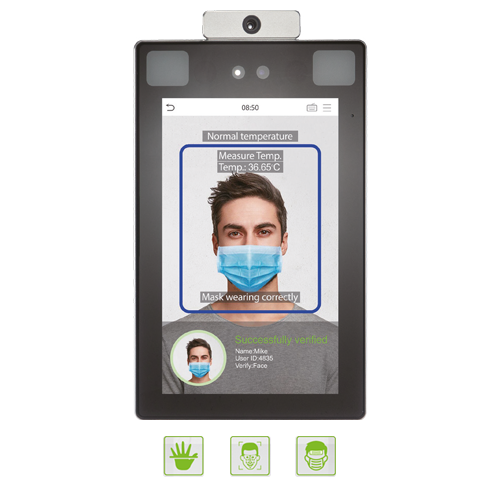
\includegraphics[trim={0.5cm 0.4cm 0.5cm 2cm},clip,width=0.80\textwidth]{gorseller/temp_image.png}
\caption{temp image}\label{fig:geofeats}
\end{figure}

\RestyleAlgo{ruled}

%% This is needed if you want to add comments in
%% your algorithm with \Comment
\SetKwComment{Comment}{/* }{ */}
\vspace{0cm}
\begin{algorithm}[htp]
\caption{x Algoirtması}\label{alg:psoudocode}
\KwData{$P$}
\KwResult{$y = [ ]$}
$y_{1} \gets [ ]$\;
$y_{2} \gets [ ]$\;
% $X \gets x$\;
$N \gets 1$\;
\While{$N \leq 68$}{
  \eIf{$N$ is even}{
    $y_{1} \gets dis(P(N),P(N+2))$\;
    $N \gets N + 1 $ \Comment*[r]{Bu aşama tekrarlanır.}
  }{\If{$N$ is odd}{
      $y_{2} \gets dis(P(N),P(N+2))$\;
      $N \gets N + 1 $ 
    }
  }
}
$y \gets y_{1} + y_{2} $
\end{algorithm}

% =========================

\newpage
\section{Alt Bölüm Birinci Derece}

\lipsum[8] \acrfull{lbp}, \acrfull{lmp}, \acrfull{ldp}, ve \acrfull{hog} 
\lipsum[6]
\acrshort{lbp}  \acrshort{hog} 
% =========================

\subsection{Alt Bölüm İkinci Derece}

\acrfull{hog}. 
\lipsum[12]. 
\acrshort{hog} 49 Şekil-\ref{flow:hog}'de gösterilmiştir. 

\begin{figure}[!htb]
    \centering
    \begin{tikzpicture}[
      >=latex',
      auto
    ]
    \node [intg] (ks)  {start};
      \node [intg] (kp) [node distance=1.8cm,below of=ks]  {nofe};
      \node [int]  (ki1) [node distance=1.5cm and -1cm,below left=of kp] {node};
      \node [int]  (ki2) [node distance=1.5cm and -1cm,below right=of kp] {node2};
      \node [intg] (hc1) [node distance=2cm,below of=ki1] {part1};
      \node [intg] (hc2) [node distance=2cm,below of=ki2] {part2};
      \node [intg] (ki3) [node distance=6.5cm,below of=kp] {share};
      \node [intg] (ki4) [node distance=2cm,below of=ki3] {final};

      \draw[->] (kp) -- ($(kp.south)+(0,-0.75)$) -| (ki1) node[above,pos=0.25] {} ;
      \draw[->] (kp) -- ($(kp.south)+(0,-0.75)$) -| (ki2) node[above,pos=0.25] {};
      \draw[->] (hc1) |- (ki3);
      \draw[->] (hc2) |- (ki3);
      \draw[->] (ki3) -- (ki4);
      \draw[->] (ks) -- (kp);
      \draw[->] (ki1) -- (hc1);
      \draw[->] (ki2) -- (hc2);
    \end{tikzpicture}
	\caption{flow chart}%\cite{paper12}.}
	\label{flow:hog}%
\end{figure}


\acrshort{hog} 
 \lipsum[12-14].

Önce $G_x$ ve $G_y$ hesaplanır. İlk $G_x$ ve $G_y$ değeri  Eşitlik-\ref{equ:hoggx}'deki formül kullanılarak hesaplanır. $r,c$ dir. $I$ asldır.

\begin{equation}
    \begin{aligned}
    G_{x}(r,c) = I(r,c+1) - I(r,c-1) 
    \\ 
    G_{y}(r,c) = I(r-1,c) - I(r+1,c) 
    \end{aligned}
 \label{equ:hoggx}
\end{equation}

$G_x$ ve $G_y$,  sonra Eşitlik-\ref{equ:hoggx2}'de sırtımsak.

\begin{equation}
    \begin{aligned}
    \textit{Büyüklük}(\mu) = \sqrt{G_{x}^{2}+G_{y}^{2}}
    \\ 
    \textit{Açı}(\theta) = \left| tan^{-1}(G_{y}/G_{x}) \right| 
    \end{aligned}
 \label{equ:hoggx2}
\end{equation}


% =========================

\newpage
\subsection{Alt Bölüm İkinci Derece2}


\lipsum[11-14]

Eşitlik-\ref{equ:lbpdistc}'de  $n$, - $t_1$, aralarındaki mesafe uzaklığı ise $d_n$ olarak gösterilmniştir.

\begin{equation}
  d_n = \sqrt{{(n_x - t_{1_x})^2}+{(n_y - t_{1_y})^2}}
 \label{equ:lbpdistc}
\end{equation}

\lipsum[5]

\begin{equation}
x = my+5 \begin{cases}
-R< i,j<R &\text{$i,j\in Z$}\\
{d_n}<R
\end{cases}
\label{equ:lbpcalc}
\end{equation}

\lipsum[6]



%\begin{equation}
\begin{equation}
    t = y^2 + x^3
    \label{eq:lbp}%
\end{equation}

\lipsum[16]

\begin{equation}
f = \sum_{i} l_{i} \begin{cases}
 0< i<68 &\text{$i\in Z$}
\end{cases}
\label{eq:4}%
\end{equation}


\chapter{BOLUM BES BUYUK BASLIK}
\lipsum[1-4]

\newpage
\section{Bölüm 5 alt başlık -1}

\lipsum[6-9]
Bu akış diyagramı detaylı olarak Şekil-\ref{fig:sffffs}'de verilmiştir. 
\lipsum[10-12]

\begin{figure}[htp]%
	\centering
    \begin{tikzpicture}[node distance=2cm]
    
    % \node (start) [startstop] {Başlama};
    \node (in1) [io2] {start};
    \node (pro1) [process2, below of=in1,yshift=-1.0cm] {check};
    \node (dec1) [decision2, below of=pro1, yshift=-3cm] {control?};
    
    \node (pro2) [process2, right of=dec1, xshift=5.0cm] {fit};
    \node (pro3) [process2, below of=dec1, yshift=-2.0cm] {finish};
    % \node (stop) [startstop, below of=out1] {Bitiş};
    
    % \coordinate (point1) at (0cm,-7.3cm);
    % \coordinate (point2) at (4.5cm,-7.3cm);
    % \coordinate (point3) at (4.5cm,-10.5cm); 
    
    % \draw [arrow] (start) -- (in1);
    \draw [arrow] (in1) -- (pro1);
    \draw [arrow] (pro1) -- (dec1);
    \draw [arrow] (pro2) |- (pro1);
    %\draw [arrow] (dec1) -- node {0.232} (pro2);
    \draw [line] (dec1) -- node[pos=0.5, anchor=south] {Yes}(pro2);
    \draw [arrow] (dec1) -- node[anchor=east] {NO} (pro3);
    % \draw [] (dec1) -- (point3);
    % \draw [arrow] (out1) -- (stop);
    
    \end{tikzpicture}
	\caption{flowchart example}%\cite{paper12}.}
	\label{fig:sffffs}%
\end{figure}


\section{Bölüm 5 alt başlık -2}

\lipsum[6-9]
Bu akış diyagramı detaylı olarak Şekil-\ref{fig:sffffs}'de verilmiştir. 
\lipsum[10-11]

\begin{figure}[htp]%
	\centering
    \begin{tikzpicture}[node distance=2cm]
    
    % \node (start) [startstop] {Başlama};
    \node (in1) [io2] {start};
    \node (pro1) [process2, below of=in1,yshift=-1.0cm] {check};
    \node (dec1) [decision2, below of=pro1, yshift=-3cm] {control?};
    
    \node (pro2) [process2, right of=dec1, xshift=5.0cm] {fit};
    \node (pro3) [process2, below of=dec1, yshift=-2.0cm] {finish};
    % \node (stop) [startstop, below of=out1] {Bitiş};
    
    % \coordinate (point1) at (0cm,-7.3cm);
    % \coordinate (point2) at (4.5cm,-7.3cm);
    % \coordinate (point3) at (4.5cm,-10.5cm); 
    
    % \draw [arrow] (start) -- (in1);
    \draw [arrow] (in1) -- (pro1);
    \draw [arrow] (pro1) -- (dec1);
    \draw [arrow] (pro2) |- (pro1);
    %\draw [arrow] (dec1) -- node {0.232} (pro2);
    \draw [line] (dec1) -- node[pos=0.5, anchor=south] {Yes}(pro2);
    \draw [arrow] (dec1) -- node[anchor=east] {NO} (pro3);
    % \draw [] (dec1) -- (point3);
    % \draw [arrow] (out1) -- (stop);
    
    \end{tikzpicture}
	\caption{flowchart example}%\cite{paper12}.}
	\label{fig:7ff7}%
\end{figure}

\newpage
\section{Bölüm 5 alt başlık - 3}
% \lipsum[1-2]
\acrfull{pca}, asdasfasf
\acrshort{pca}'
\lipsum[3]
\parencite{cheng_principal_2022} tarafından yayınlanan Şekil-\ref{fig:apcaaaa} 
\lipsum[15]

\begin{figure}[hbp]
\centering
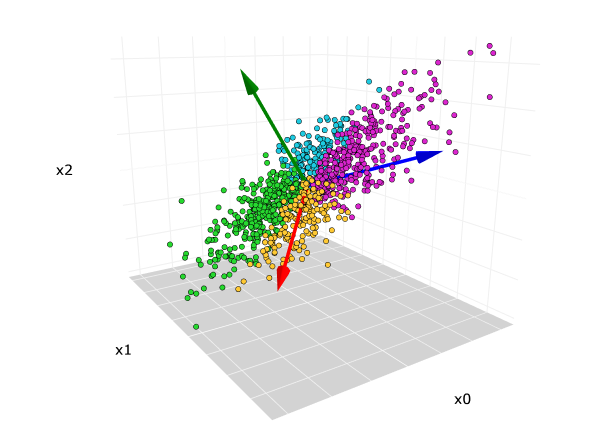
\includegraphics[width=0.69\textwidth]{gorseller/pca_desc.png}
\caption{\acrlong{pca} image}\label{fig:apcaaaa}
\end{figure}

\chapter{BOLUM ALTI BUYUK BASLIK}
\lipsum[1-2]
\acrlong{svm} , \acrlong{rf}, \acrlong{logreg}  ve \acrlong{cva}dır.

\section{Bölüm 6 alt başlık - bir}
\lipsum[3-4]
\acrfull{svm}  
\parencite{Hearst1998} 
\lipsum[6-8]
\acrshort{svm},  
$n$-\lipsum[11]

\begin{equation}
\overrightarrow{W}x_{i}+b = 0
\label{eq:ssss}%
\end{equation}

Eşitlik-\ref{eq:ssss}'de verilen $\overrightarrow{W}$ sd, $x_{i}$ olarak da supplyri, $b$ is değeri göstermektedir.

\lipsum[4]

\section{Bölüm 6 alt başlık - iki}
\lipsum[1-2]

\acrfull{rf}, 
\lipsum[8-10]


\begin{figure}[htp]
\centering
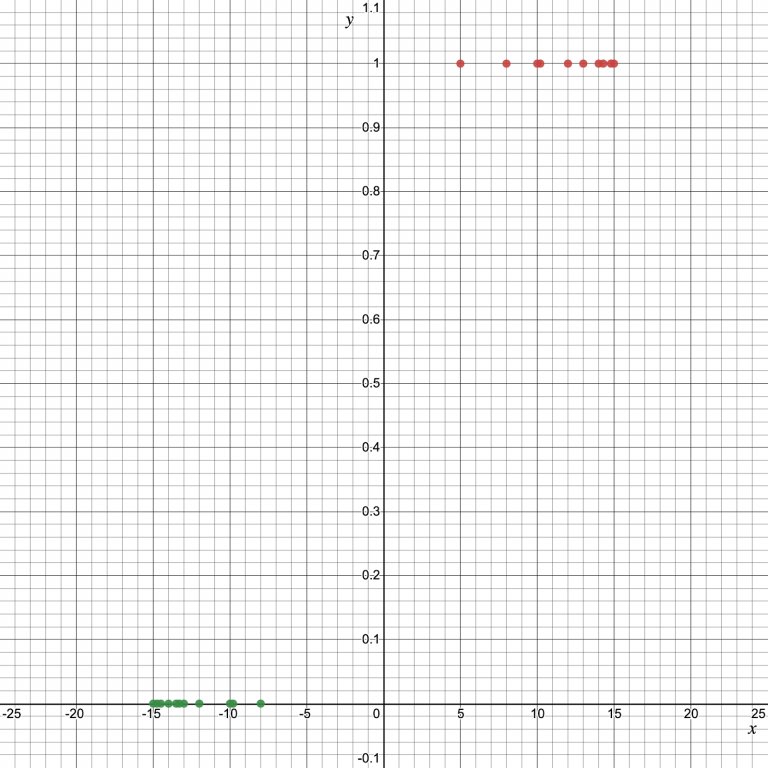
\includegraphics[width=0.69\textwidth]{gorseller/graph1.png}
\caption{yapnın yapısı}\label{fig:randomforest}
\end{figure}

\acrshort{rf}

\lipsum[3]

\addtocontents{toc}{~\hfill\underline{\textbf{Sayfa}}\vspace{0.3cm}\par} %% TODO: SAYFA YAZISI
% Cilt onay için reddedildikten sonra içerikteki ikinci kısma eklemek için dahil edildi.
\section{Bölüm 6 alt başlık - üç}
 \lipsum[1-2]



\acrfull{logreg} 
\lipsum[5]
Şekil-\ref{fig:ghsakjh}'de verilmiştir.  

\begin{figure}[htp]
\centering
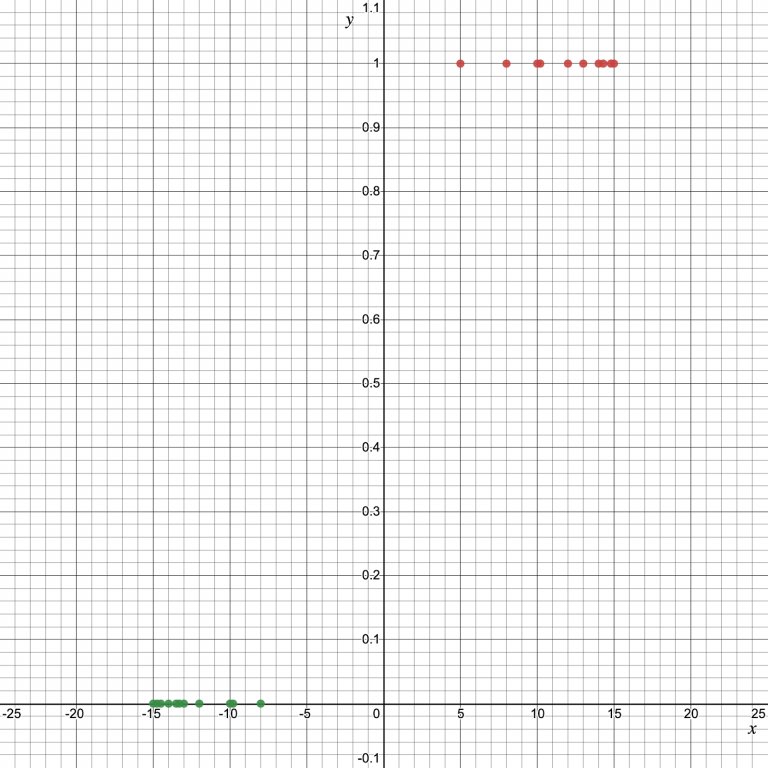
\includegraphics[width=0.45\textwidth]{gorseller/graph1.png}
\caption{Veri kümesindeki özniteliklerin düzlemdeki dağılımı}\label{fig:ghsakjh}
\end{figure}

 Eşitlik-\ref{eq:sadasfas}'dek

\begin{equation}
y = \frac{1}{(1+e^{-x})}
\label{eq:sadasfas}%
\end{equation}

\begin{figure}[htp]
\centering
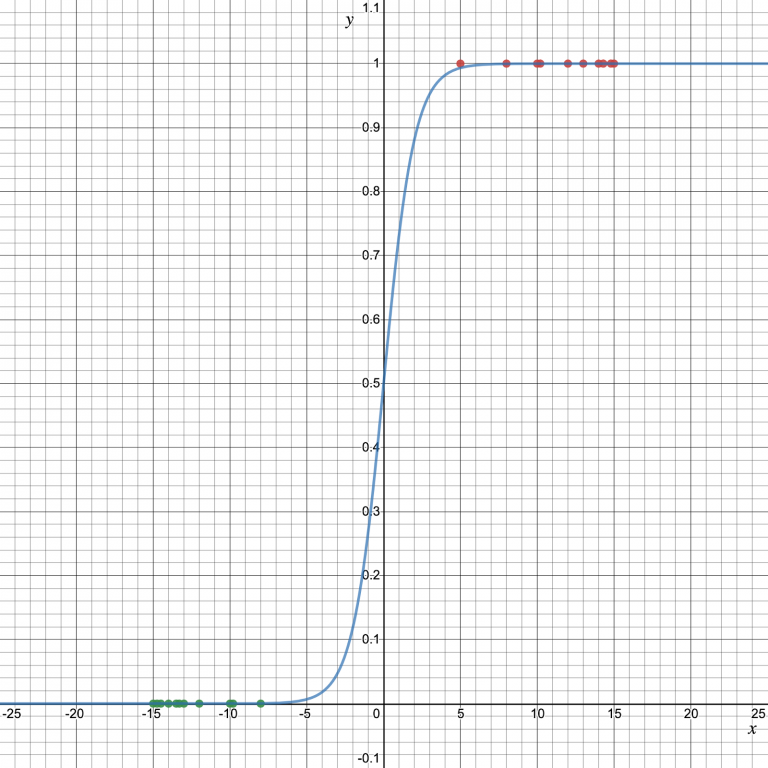
\includegraphics[width=0.45\textwidth]{gorseller/graph2.png}
\caption{Öznitelikler üzerine yerleştirilmiş sigmoid fonksiyonu}\label{fig:ghsakjh2}
\end{figure}

\lipsum[24]
\newpage
\section{Bölüm 6 alt başlık - dört}
% \lipsum[1-2]

\acrfull{cva}

\vspace{0.5cm}
\subsection{Bölüm 6 alt başlık - dört - alt başlık - 1}

\lipsum[10-12]

\subsection{Bölüm 6 alt başlık - dört - alt başlık - 2}

\lipsum[14-16]
\begin{figure}[htp]
\caption{PTA Torç}\label{fig:PtaTorc1}
\end{figure}
\begin{figure}[htp]
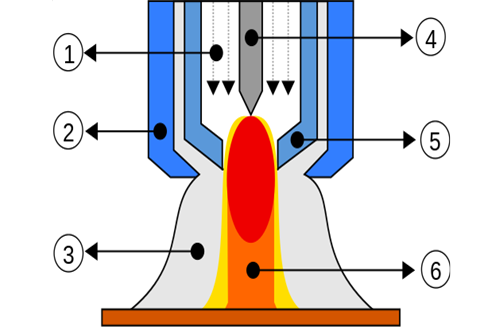
\includegraphics[width=\textwidth]{gorseller/ptaTorc}
\caption{PTA Torç}\label{fig:PtaTorc2}
\end{figure}
\begin{figure}[htp]
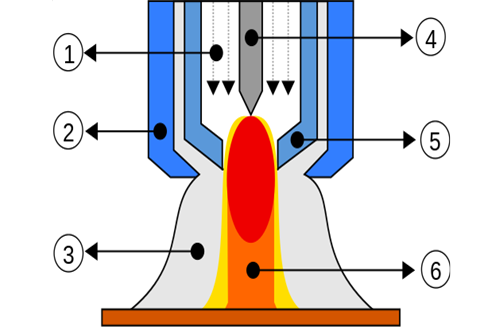
\includegraphics[width=\textwidth]{gorseller/ptaTorc}\centering
\centering
\centering
\centering

\caption{PTA Torç}\label{fig:PtaTorc3}
\end{figure}
\begin{figure}[htp]
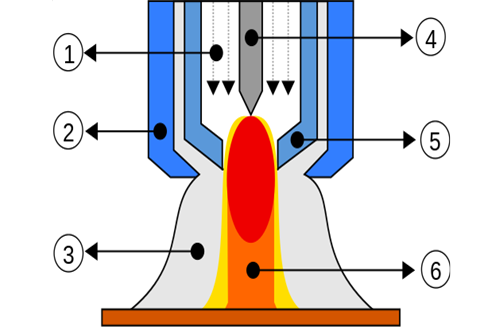
\includegraphics[width=\textwidth]{gorseller/ptaTorc}
\caption{PTA Torç}\label{fig:PtaTorc4}
\end{figure}
\begin{figure}[htp]
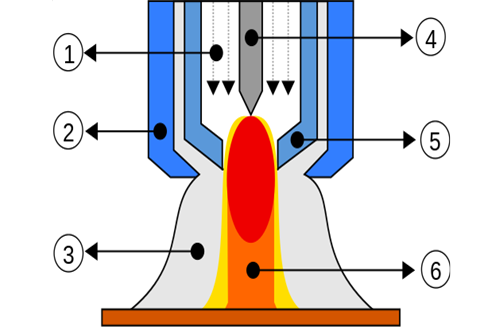
\includegraphics[width=\textwidth]{gorseller/ptaTorc}
\caption{PTA Torç}\label{fig:PtaTorc5}
\end{figure}
\begin{figure}[htp]
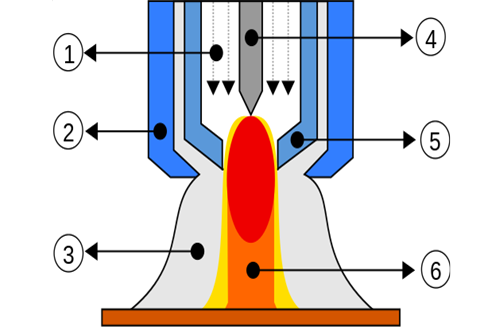
\includegraphics[width=\textwidth]{gorseller/ptaTorc}
\caption{PTA Torç}\label{fig:PtaTorc6}
\end{figure}
\begin{figure}[htp]
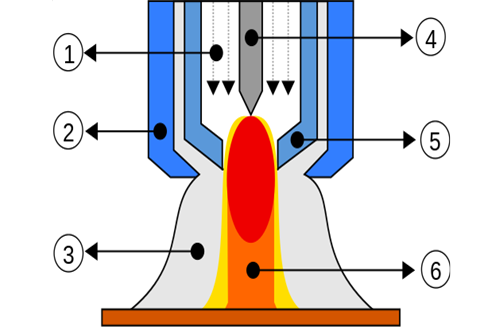
\includegraphics[width=\textwidth]{gorseller/ptaTorc}
\caption{PTA Torç}\label{fig:PtaTorc7}
\end{figure}\begin{figure}[htp]
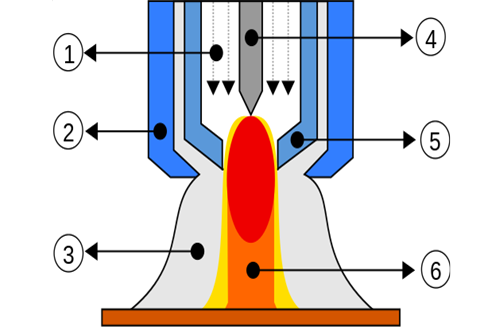
\includegraphics[width=\textwidth]{gorseller/ptaTorc}
\caption{PTA Torç}\label{fig:PtaTorc8}
\end{figure}
\begin{figure}[htp]
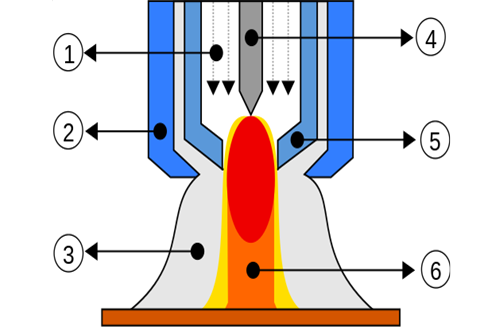
\includegraphics[width=\textwidth]{gorseller/ptaTorc}
\caption{PTA Torç}\label{fig:PtaTorc9}
\end{figure}
\begin{figure}[htp]
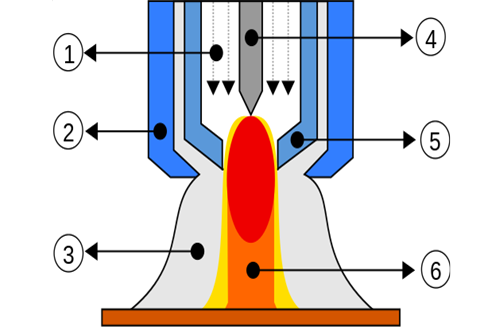
\includegraphics[width=\textwidth]{gorseller/ptaTorc}
\caption{PTA Torç}\label{fig:PtaTorc10}
\end{figure}
\begin{figure}[htp]
\caption{PTA Torç}\label{fig:PtaTorc11}
\end{figure}


vfj ndsobvsfobşvjnsfbvs
 sjfdb s
\lipsum 

\begin{figure}[htp]
\caption{PTA Torç}\label{fig:PtaTorc12}
\end{figure}
\begin{figure}[htp]
\caption{PTA Torç}\label{fig:PtaTorc13}
\end{figure}

vrebvsfdbsdbf

\section{deneme}

cdsvefvfdv
\begin{figure}[htp]
\caption{PTA Torç}\label{fig:PtaTorc14}
\end{figure}
\chapter{Bolüm}
\begin{figure}[htp]
\caption{PTA Torç}\label{fig:PtaTorc15}
\end{figure}
\section{deneme34g}
\begin{figure}[htp]
\caption{PTA Torç}\label{fig:PtaTorc16}
\end{figure}
\begin{figure}[htp]
\caption{PTA Torç}\label{fig:PtaTorc17}
\end{figure}

\begin{figure}[htp]
\caption{PTA Torç}\label{fig:PtaTorc18}
\end{figure}
\chapter{BULGULAR VE TARTIŞMA}

Basit iki terimle \acrfull{lbp} ve \acrfull{hog} kısaltmaları anlatabiliriz. İster kısaltmasını \acrshort{lbp}, isterseniz de uzun açılımını \acrlong{hog} yazdırabilirsiniz. Bunu yapabilmek için dosyanın başında terimleri tanımlamanız gereklidir. İsterseniz matematik terimlerini de, örneğin \acrshort{fer} böyle tanımlayabilirsiniz. Uzun uzun \acrfull{fer} yazmanız gerekmez. 

\lipsum[19-25]

\section{section-name-1}

Öznitelik vektörleri oluşturulurken öncelikli olarak imge üzerinden yüz tespit edilmesi ve yüz üzerine 68 nirengi noktasının yerleştirmesiyle başlamıştır. Devam eden alt bölümlerde bu nirengi noktalarının görünüm ve geometrik olarak nasıl kullanıldığına yer verilecektir.

\subsection{subsection-name-1}

Eşitlik-\ref{eq:result_geo}’de verilen formüle 
\lipsum[2]


%eşitlik.
\begin{equation}
F_{x } =2 \times \frac{(n_{1})\times(n_{1}-1)}{2}  
\label{eq:result_geo}%
\end{equation}

\subsection{subsection-name-2}

\acrfull{hog} 
\lipsum[30]

%eşitlik.
\begin{equation}
F_{ x } = ((s_{row}/b_{row}) - c_{row} +1) \times ((s_{col} / b_{col}) - c_{col} +1) \times c_{row} \times c_{col} \times y
\label{eq:result_hog}%
\end{equation}


\subsection{subsection-name-3}

\acrlong{lbp} \lipsum[3]
%eşitlik.
\begin{equation}
F_{ \text{THETA} } = (n_{1} \times n_{2})
\label{eq:result_lbp}%
\end{equation}

\section{section-name-2}

\lipsum[22-25]
Tablo-\ref{tab:featuresize} de verilmiştir. 

\begin{table}[hpb]
    \centering
    \caption{Öznitelik çıkarım yöntemine göre boyut indirgenmiş öznitelik sayıları}
    \begin{tabular}{ |p{4.5cm}||p{2.5cm}|p{2.5cm}|p{2.5cm}|  }
     \hline
     \multicolumn{4}{|c|}{Öznitelik Sayıları} \\
     \hline
     Öznitelik Seçim Yöntemi& Geometrik & YGH & YİÖ\\
     \hline
     Temel Öznitelikler   & 1122    &2800&   17408\\
     \acrshort{sffs} &   60  & 171   &7680\\
     \acrshort{sbfs} & 28 & 195&  5888\\
     \acrshort{pca} & 268 & 268&  866\\
     \hline
    \end{tabular}
    \label{tab:featuresize}
\end{table}

\lipsum[3]

\section{section-name-3}

\lipsum[1-2]

\section{Deney Sonuçları}


 Çizelge-\ref{tab:smotetablo}'de 
 \lipsum[3]

\subsection{Final-Subsection-1}

Geometrik öznitelikleri için \acrshort{svm}, \acrshort{rf} ve \acrshort{logreg} sınıflandırıcıları ile sınıflandırma sonuçları  Şekil-\ref{fig:ckrawgeoall}'te verilmiştir. 

\begin{figure}[hbt!]

\begin{subfigure}{.475\linewidth}
  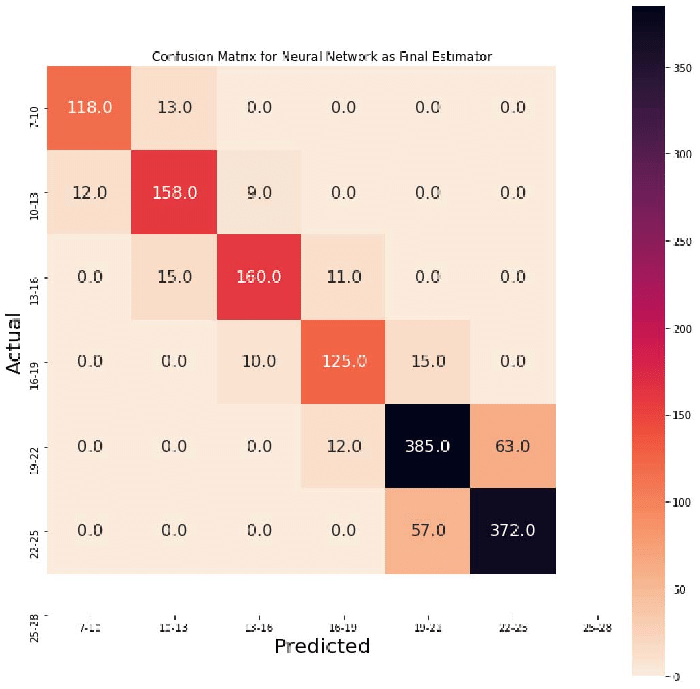
\includegraphics[trim={0 0 0 0.72cm},clip,width=\linewidth]{gorseller/Confusion-Matrix.png}
  \caption{DVM-$rbf$}
  \label{MLEDdet0}
\end{subfigure}\hfill % <-- "\hfill"
\begin{subfigure}{.475\linewidth}
  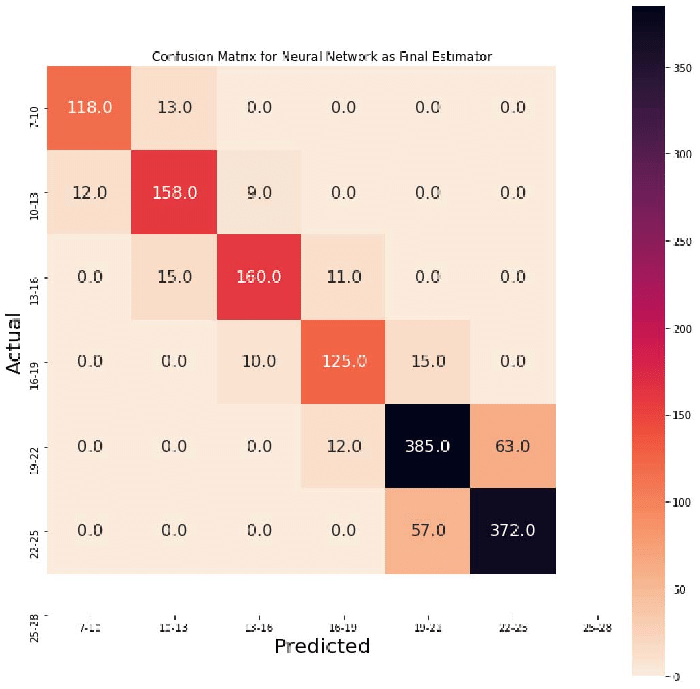
\includegraphics[trim={0 0 0 0.72cm},clip,width=\linewidth]{gorseller/Confusion-Matrix.png}
  \caption{DVM-$\textit{doğrusal}$}
  \label{energydetPSK0}
\end{subfigure}

\medskip % create some *vertical* separation between the graphs
\begin{subfigure}{.475\linewidth}
  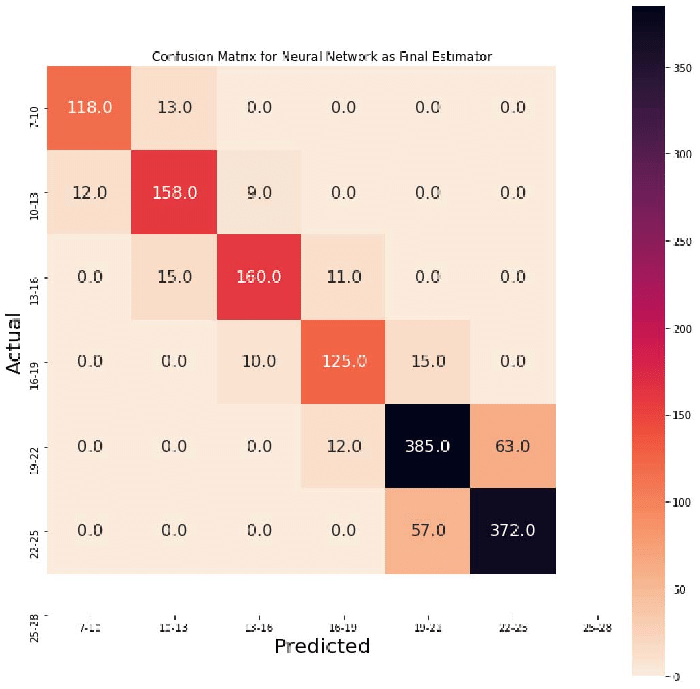
\includegraphics[trim={0 0 0 0.72cm},clip,width=\linewidth]{gorseller/Confusion-Matrix.png}
  \caption{RO}
  \label{velcomp0}
\end{subfigure}\hfill % <-- "\hfill"
\begin{subfigure}{.475\linewidth}
  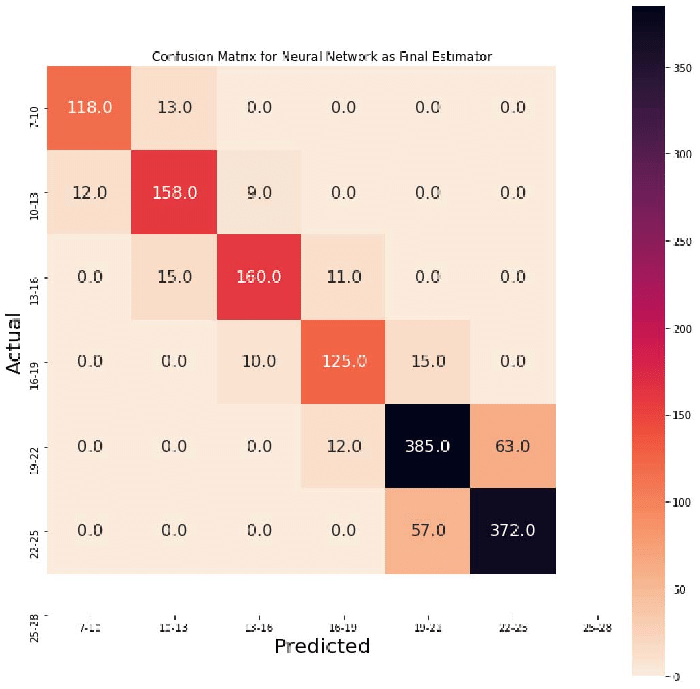
\includegraphics[trim={0 0 0 0.72cm},clip,width=\linewidth]{gorseller/Confusion-Matrix.png}
  \caption{LRC}
  \label{estcomp0}
\end{subfigure}

\caption{tab 2}
\label{fig:ckrawgeoall}
\end{figure}


\lipsum[4] 
Şekil-\ref{fig:ckrawgeoall}'te yer verilmiştir.

%Ssad


\begin{figure}[hbt!]

\begin{subfigure}{.475\linewidth}
  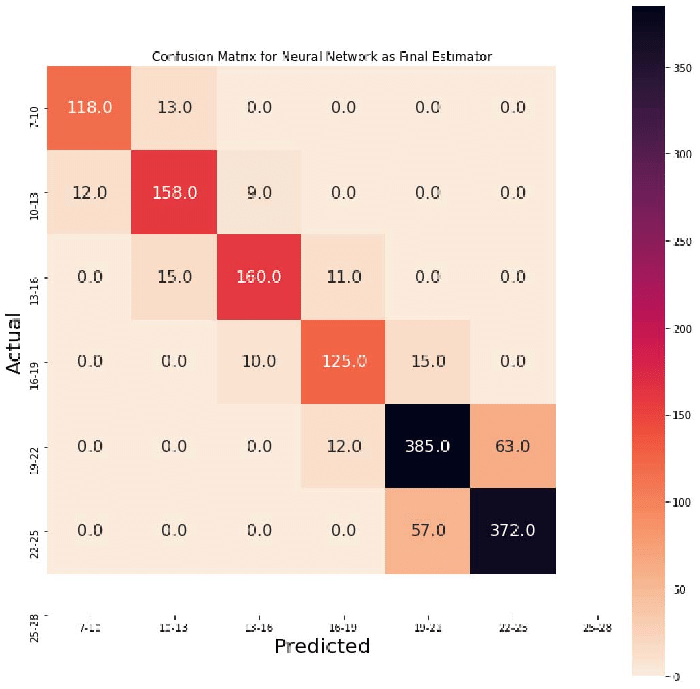
\includegraphics[trim={0 0 0 0.72cm},clip,width=\linewidth]{gorseller/Confusion-Matrix.png}
  \caption{DVM-$rbf$}
  \label{MLEDdet1}
\end{subfigure}\hfill % <-- "\hfill"
\begin{subfigure}{.475\linewidth}
  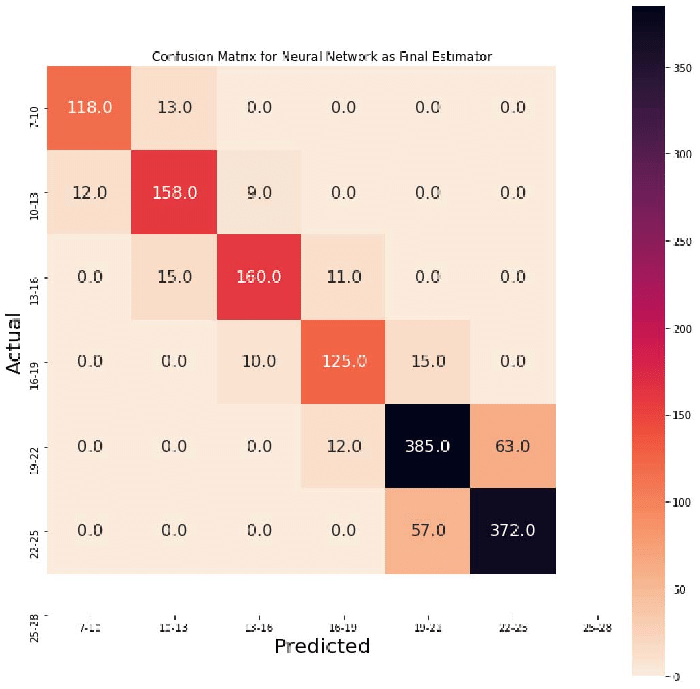
\includegraphics[trim={0 0 0 0.72cm},clip,width=\linewidth]{gorseller/Confusion-Matrix.png}
  \caption{DVM-$\textit{doğrusal}$}
  \label{energydetPSK1}
\end{subfigure}

\medskip % create some *vertical* separation between the graphs
\begin{subfigure}{.475\linewidth}
  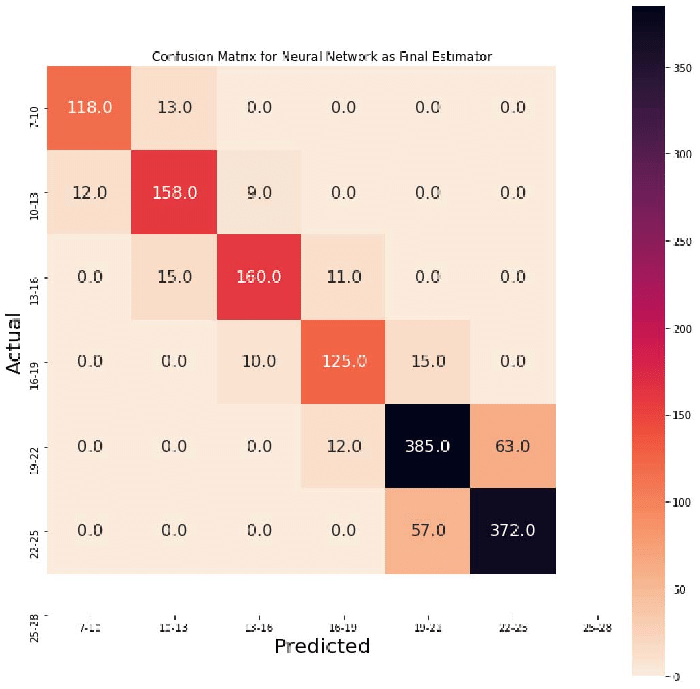
\includegraphics[trim={0 0 0 0.72cm},clip,width=\linewidth]{gorseller/Confusion-Matrix.png}
  \caption{RO}
  \label{velcomp1}
\end{subfigure}\hfill % <-- "\hfill"
\begin{subfigure}{.475\linewidth}
  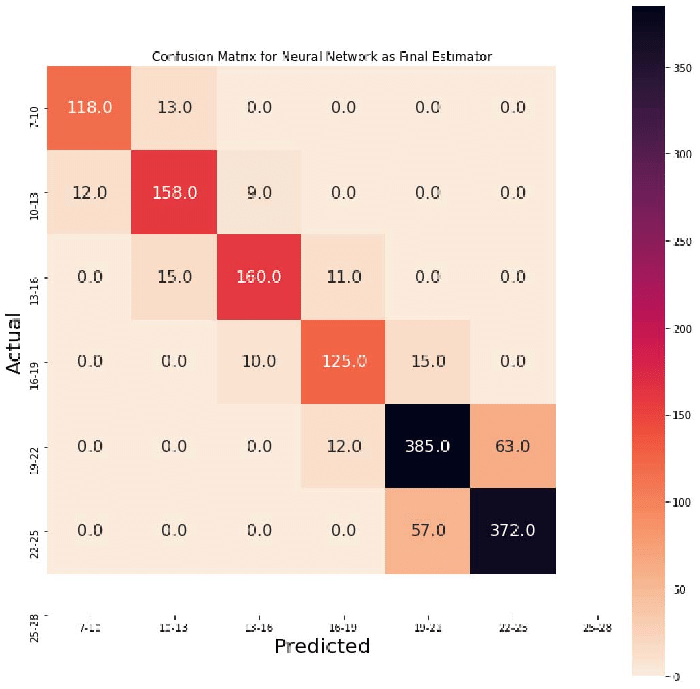
\includegraphics[trim={0 0 0 0.72cm},clip,width=\linewidth]{gorseller/Confusion-Matrix.png}
  \caption{LRC}
  \label{estcomp1}
\end{subfigure}

\caption{sdaafsfa}
\label{fig:cksffsgeoall}
\end{figure}

% \begin{figure}[hbp]
% \centering
% \includegraphics[trim={0 0 0 0.72cm},clip,width=0.53\textwidth]{conf_mat/conf_mat_geometric_sffs_rbf_SVM.png}
% \caption{AİÖS uygulanmış geometrik özniteliklerin DVM-$rbf$ çekirdeğindeki karmaşıklık matrisi}\label{fig:conf_mat_geometric_sffs_rbf_SVM}
% \end{figure}

% \begin{figure}[hp]
% \centering
% \includegraphics[trim={0 0 0 0.72cm},clip,width=0.53\textwidth]{conf_mat/conf_mat_geometric_sffs_Linear_SVM.png}
% \caption{AİÖS uygulanmış geometrik özniteliklerin DVM-$\textit{doğrusal}$ çekirdeği ile karmaşıklık matrisi}\label{fig:conf_mat_geometric_sffs_Linear_SVM}
% \end{figure}

% \begin{figure}[hp]
% \centering
% \includegraphics[trim={0 0 0 0.72cm},clip,width=0.53\textwidth]{conf_mat/conf_mat_geometric_sffs_Random_Forest.png}
% \caption{AİÖS uygulanmış geometrik özniteliklerin RO ile  karmaşıklık matrisi}\label{fig:conf_mat_geometric_sffs_Random_Forest}
% \end{figure}

% \begin{figure}[hp]
% \centering
% \includegraphics[trim={0 0 0 0.72cm},clip,width=0.53\textwidth]{conf_mat/conf_mat_geometric_sffs_Logistic_Regression.png}
% \caption{AİÖS uygulanmış geometrik özniteliklerin LRS ile karmaşıklık matrisi}\label{fig:conf_mat_geometric_sffs_Logistic_Regression}
% \end{figure}



% \begin{figure}[hbp]
% \centering
% \includegraphics[trim={0 0 0 0.72cm},clip,width=0.53\textwidth]{conf_mat/conf_mat_geometric_sbfs_rbf_SVM.png}
% \caption{AGÖS uygulanmış geometrik özniteliklerin DVM-$rbf$ çekirdeğindeki karmaşıklık matrisi}\label{fig:conf_mat_geometric_sbfs_rbf_SVM}
% \end{figure}

% \begin{figure}[hp]
% \centering
% \includegraphics[trim={0 0 0 0.72cm},clip,width=0.53\textwidth]{conf_mat/conf_mat_geometric_sbfs_Linear_SVM.png}
% \caption{AGÖS uygulanmış geometrik özniteliklerin DVM-$\textit{doğrusal}$ çekirdeği ile karmaşıklık matrisi}\label{fig:conf_mat_geometric_sbfs_Linear_SVM}
% \end{figure}

% \begin{figure}[htbp]
% \centering
% \includegraphics[trim={0 0 0 0.72cm},clip,width=0.53\textwidth]{conf_mat/conf_mat_geometric_sbfs_Random_Forest.png}
% \caption{AGÖS uygulanmış geometrik özniteliklerin RO ile  karmaşıklık matrisi}\label{fig:conf_mat_geometric_sbfs_Random_Forest}
% \end{figure}

% \begin{figure}[htbp]
% \centering
% \includegraphics[trim={0 0 0 0.72cm},clip,width=0.53\textwidth]{conf_mat/conf_mat_geometric_sbfs_Logistic_Regression.png}
% \caption{AGÖS uygulanmış geometrik özniteliklerin LRS ile karmaşıklık matrisi}\label{fig:conf_mat_geometric_sbfs_Logistic_Regression}
% \end{figure}

% \lipsum[1]

% \begin{figure}[htbp]
% \centering
% \includegraphics[trim={0 0 0 0.72cm},clip,width=0.53\textwidth]{conf_mat/conf_mat_geometric_pca_rbf_SVM.png}
% \caption{TBA öznitelik seçimi uygulanmış geometrik özniteliklerin DVM-$rbf$ çekirdeğindeki karmaşıklık matrisi}\label{fig:conf_mat_geometric_pca_rbf_SVM}
% \end{figure}

% \begin{figure}[htbp]
% \centering
% \includegraphics[trim={0 0 0 0.72cm},clip,width=0.53\textwidth]{conf_mat/conf_mat_geometric_pca_Linear_SVM.png}
% \caption{TBA öznitelik seçimi uygulanmış geometrik özniteliklerin DVM-$\textit{doğrusal}$ çekirdeği ile karmaşıklık matrisi}\label{fig:conf_mat_geometric_pca_Linear_SVM}
% \end{figure}

% \begin{figure}[htbp]
% \centering
% \includegraphics[trim={0 0 0 0.72cm},clip,width=0.53\textwidth]{conf_mat/conf_mat_geometric_pca_Random_Forest.png}
% \caption{TBA öznitelik seçimi uygulanmış geometrik özniteliklerin RO ile  karmaşıklık matrisi}\label{fig:conf_mat_geometric_pca_Random_Forest}
% \end{figure}

% \begin{figure}[htbp]
% \centering
% \includegraphics[trim={0 0 0 0.72cm},clip,width=0.53\textwidth]{conf_mat/conf_mat_geometric_pca_Logistic_Regression.png}
% \caption{TBA öznitelik seçimi uygulanmış geometrik özniteliklerin LRS ile karmaşıklık matrisi}\label{fig:conf_mat_geometric_pca_Logistic_Regression}
% \end{figure}


\clearpage
\newpage
\lipsum[5]
Çizelge-\ref{tab:ckgeometrikacc}'de verilmiştir. 
\lipsum[6]



\begin{table}[hpt]
    \centering
    \caption{sınıflandırma Sonuçları}
    \begin{tabular}{ |p{3cm}||p{3cm}|p{2.5cm}|p{2.5cm}|  }
     \hline
     \multicolumn{4}{|c|}{ ccccccc test} \\
     \hline
     \hline
     feats & cccccc &X1 & X2\\
     \hline
     \hline
     \multirow{5}{4em}{feat3} & XXX-$\textit{ll}$ & 0.8821 &	0.9836 \\ 
         & ddd-$rbf$ & 0.8474 &	0.9570
  \\ 
         & rrr & 0.7782&	0.9423
 \\ 
         & lll & 0.9145	&\textbf{0.9854}
 \\ 
         & ooo & 0.6982&	0.9250
\\
     \hline
     \multirow{5}{4em}{feat2} & XXX-$\textit{ll}$ & 0.8695&	0.9639
\\ 
         & ddd-$rbf$ & 0.8915&	0.9544
 \\ 
         & rrr & 0.8048&	0.9381
\\ 
         & lll & 0.8834&	0.9621
\\ 
         & ooo & 0.8236	&0.9232
\\
     \hline
     \multirow{5}{4em}{feat1} & XXX-$\textit{ll}$ & 0.9272&	0.9803
\\ 
         & ddd-$rbf$ & \textbf{0.9352}&	0.9578
\\ 
         & rrr & 0.7991&	0.9382
\\ 
         & lll & 0.9157&	0.9750
\\ 
         & ooo & 0.8375&	0.8991
\\
     \hline
     \multirow{5}{4em}{feat} & XXX-$\textit{ll}$ & 0.8901&	0.9845
\\ 
         & ddd-$rbf$ & 0.8326&	0.9527
 \\ 
         & rrr & 0.8060&	0.9441
\\ 
         & lll & 0.9086&	0.9837
\\ 
         & ooo & 0.7169&	0.9384
\\
     \hline
    \end{tabular}
    \label{tab:ckgeometrikacc}
\end{table}


\subsection{Final-Subsection-2}

\lipsum[1-2]



% ==========================================

% ==========================================
\subsection{Final-Subsection-3}

\lipsum[4-6]



% ====================================

\subsection{Final-Subsection-4}
\lipsum[10-11]
% ===========================================================================
% ===========================================================================
% ===========================================================================
\newpage
\subsection{Final-Subsection-5}
\lipsum[12-13]
\chapter{SONUÇ VE ÖNERİLER}

\lipsum[14-22]


\newpage

\newcommand\MyShipoutHookn{\chapter*{KAYNAKLAR\space DİZİNİ \MakeLowercase{{ (devam)}}}}

\AtBeginShipout{\MyShipoutHookn}
\printbibliography[ title={KAYNAKLAR\space DİZİNİ}]
\renewcommand\MyShipoutHookn{}
%numaralı olsun istersen optionlarda heading=bibnumbered, yaz
\defbibheading{bibliography}[\refname]{%
  \section*{#1}%
  \markboth{\MakeUppercase{#1}}{\MakeUppercase{#1}}}
  
% \chapter{EK AÇIKLAMALAR}  
% \section{Ek Açıklamalar}
%\cftaddtitleline{toc}{chapter}{\textbf{Özgeçmiş}}{}   % Sadece doktora tezleri için

\end{document}